 % Tarea 1 Electro





% PROBLEMA 1
\begin{mdframed}[style = warning]
	\begin{problem}
		Utilizando la definición de campo eléctrico:
			$$\vec{E} = \frac{1}{4\pi \varepsilon _o}\int \frac{\dd{q}}{r^2}$$
		Además, por simetría, las componentes $x,y$ del campo son cero, ademas, la componente $z$, es $4$ veces la contribución de un lado del cuadrado. Tomando unicamente un lado del cuadrado se tiene que la distancia de la carga al punto es: $r = z\vz - \frac{l}{2} \vy - x\vx$, con lo que:
			$$\vec{E} _1 = \frac{1}{4\pi \varepsilon _o} \int _{-\flatfrac{l}{2}} ^{\flatfrac{l}{2}} \frac{\lambda}{x^2 + z^2 + \flatfrac{l^2}{4}} \frac{z\vz - \frac{l}{2} \vy - x\vx}{\sqrt{x^2 + z^2 + \flatfrac{l^2}{4}}} \dd{x}$$
		Unicamente integrando la componente $z$, utilizando herramientas computacionales:
			$$ = \frac{z\lambda}{4\pi \varepsilon _o} \frac{1}{z^2 + \flatfrac{l^2}{4}} \frac{l}{\sqrt{z^2 + \flatfrac{l^2}{2}}}$$
		Sumando las $4$ contribuciones se tiene:
			$$\boxed{\vec{E} _z = \frac{4z\lambda}{\pi \varepsilon _o} \frac{1}{4z^2 + l^2} \frac{l}{\sqrt{z^2 + \flatfrac{l^2}{2}}} \vz}$$
	\end{problem}
\end{mdframed}







% PROBLEMA 2
\begin{mdframed}[style = warning]
	\begin{problem}
		Como en la región dentro de ambas esferas no hay carga, se utiliza Laplace en $1$ y, por simetría esférica, se tiene:
			$$\nabla ^2 \varphi = 0 \quad \quad \varphi (r) = -\frac{a}{r} + b$$
		Condiciones de frontera:
		\begin{multicols}{2}
			$$\varphi (r_a) = \varphi _a = -\frac{a}{r_a} + b$$
			\columnbreak
			$$\varphi (r_b) = \varphi _b = -\frac{a}{r_b} + b$$
		\end{multicols}
		Resolviendo el sistema de ecuaciones, se tiene que:
			$$a = \frac{\varphi _b - \varphi _a}{r_b - r_a} r_a r_b$$
			$$b = \frac{\varphi _b r_b - \varphi _a r_a}{r_b - r_a}$$
		Sustituyendo, se encuentra el potencial entre las dos esferas concéntricas:
			$$\boxed{\varphi (r) = \frac{\varphi _b - \varphi _a}{r_b - r_a} \frac{r_a r_b}{r} + \frac{\varphi _b r_b - \varphi _a r_a}{r_b - r_a}}$$
	\end{problem}
\end{mdframed}






% PROBLEMA 3
\begin{mdframed}[style = warning]
	\begin{problem}
		Como el sistema de referencia se colocará de modo que haga los cálculos más simples, por lo que se coloca la carga en el eje $z$ donde su posición relativa al origen es mayor al radio de la esfera. Con esto, es claro que el campo dependerá de la distancia y del ángulo respecto a $z$. Por simetría esférica, se utiliza la solución a la ecuación de Laplace:
			$$\varphi (r,\theta) = \sum _{n=0} ^\infty \qty(A_n r^n + B_n r^{-(n+1)}) P_n (\cos{\theta})$$
		Por limitaciones físicas $A_2 ,\ldots = 0$ para que el potencial no diverja en el infinito; además, $B_2,\ldots \to 0$ por los términos $r^{-(n+1)}$. Con esto, se tiene:
			$$\varphi (r,\theta) = A_o \frac{B_o}{r} + A_1 r\cos{\theta} + \frac{B_1}{r^2} \cos{\theta}$$
		Encontrando el potencial fuera de la esfera debido a los campos eléctricos, integrando:
			$$\varphi = -\int (E_o + E_Q)\cdot \dd{r} = -\int E_o \cos{\theta} \dd{r} - \int \frac{kQ}{r^2} \dd{r} = -E_o r\cos{\theta} + \frac{1}{4\pi \varepsilon _o} \frac{Q}{r}$$
		Con lo que se tienen las constantes $B_o = \frac{Q}{4\pi \varepsilon _o}$ y $A_1 = -E_o$. El potencial es igual a cero, cuando se cumplan las condiciones $r\to \infty$ y $\theta = \flatfrac{(2k + 1)\pi}{2}, \, k=0,\ldots$, lo que claramente es cierto, puesto que para multiplos impares de $\flatfrac{\pi}{2}$ se elimina la contribución constante del campo externo, por lo que $\varphi (r\to \infty ,\theta = \flatfrac{(2k + 1)\pi}{2}) = A_o = 0$. Con esto, el término restante es la aportación dipolar. Utilizando la condición en la cual se tiene $r = R$ el potencial debe ser igual al de la carga puntual, entonces:
			$$\frac{1}{4\pi \varepsilon _o} \frac{Q}{R} = \frac{1}{4\pi \varepsilon _o} \frac{Q}{R} - E_o R \cos{\theta} + \frac{B_1}{R^2} \cos{\theta}$$
		Con lo que $B_1 = E_o R^3$; el potencial fuera de la esfera cargada sumregida en un campo eléctrico constante:
			$$\boxed{\varphi (r,\theta) = \frac{1}{4\pi \varepsilon _o} \frac{Q}{r} - E_o \qty(r + \frac{R^3}{r^2}) \cos{\theta}}$$
	\end{problem}
\end{mdframed}







% PROBLEMA 4
\begin{mdframed}[style = warning]
	\begin{problem}
		Tomando el campo eléctrico dado, utilizando la Ley de Gauss en forma diferencial se tiene:
			$$\div{\vec{E}} = \frac{\rho}{\varepsilon _o}$$
		Entonces:
			$$\pdv{r} \qty(A\frac{e^{-rb}}{r}) = \frac{\rho}{\varepsilon _o}$$
		Despejando la densidad de carga volumétrica:
			$$\boxed{\rho (r) = -A\varepsilon _o e^{-br} \qty(\frac{1}{r^2} + \frac{b}{r})}$$
	\end{problem}
\end{mdframed}








% PROBLEMA 5
\begin{mdframed}[style = warning]
	\begin{problem}
		Para encontrar los puntos en los cuales el campo es cero, se encuentra el potencial en cualquier punto por contribución de las $n$ cargas puntuales colocadas en los vértices del poligono regular.
		\begin{description}
			\item[Para $n = 3$: ] Se tiene que el potencial si se toma la figura como en la figura \ref{TP5}.
			\begin{figure}[H]
				\centering
				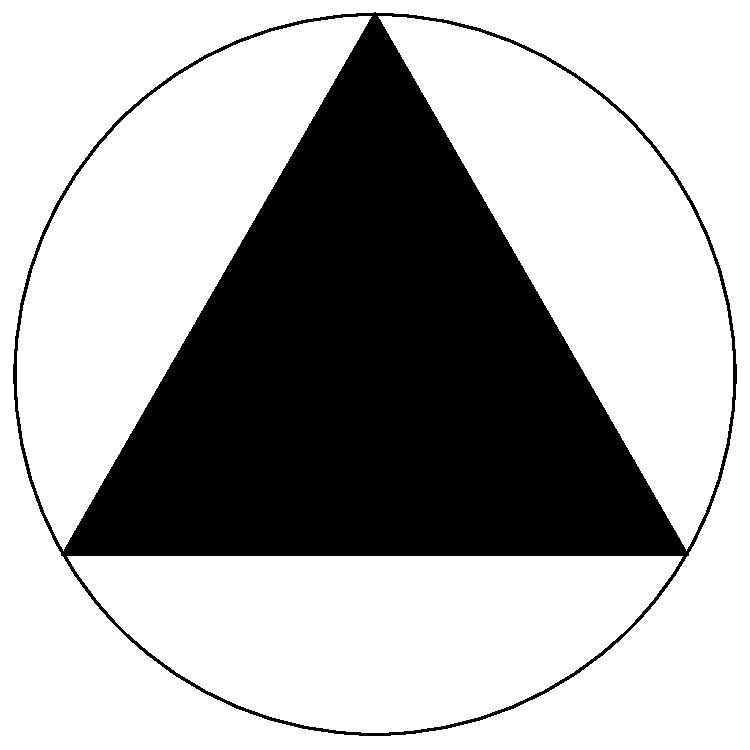
\includegraphics[scale=0.5]{Images/TriangleP5.pdf}
				\caption{Triángulo Inscrito en una Circunferecia, creado con \textit{Mathematica}.}
				\label{TP5}
			\end{figure}
			De modo que, el potencial debido a dichas cargas, en cualquier punto del espacio es:
				$$\phi (x,y) = \frac{q}{4\pi \varepsilon _o} \qty[\frac{1}{\sqrt{(y-a)^2+x^2}}+\frac{1}{\sqrt{\left(x-\frac{\sqrt{3} a}{2}\right)^2+\left(\frac{a}{2}+y\right)^2}}+\frac{1}{\sqrt{\left(\frac{\sqrt{3} a}{2}+x\right)^2+\left(\frac{a}{2}+y\right)^2}}]$$
			Con esto, se aplica la relación entre el campo eléctrico y el potencial $\vec{E} = -\grad{\phi}$, de modo que, el campo es:
				$$ \vec{E} = \frac{-q}{4\pi \varepsilon _o} \left(-\frac{x}{\left((a-y)^2+x^2\right)^{3/2}}-\frac{\frac{\sqrt{3} a}{2}+x}{\left(\left(\frac{\sqrt{3} a}{2}+x\right)^2+\left(\frac{a}{2}+y\right)^2\right)^{3/2}}-\frac{x-\frac{\sqrt{3} a}{2}}{\left(\left(x-\frac{\sqrt{3} a}{2}\right)^2+\left(\frac{a}{2}+y\right)^2\right)^{3/2}}\right)\vx$$
				
				$$\left(\frac{a-y}{\left((a-y)^2+x^2\right)^{3/2}}-\frac{\frac{a}{2}+y}{\left(\left(\frac{\sqrt{3} a}{2}+x\right)^2+\left(\frac{a}{2}+y\right)^2\right)^{3/2}}-\frac{\frac{a}{2}+y}{\left(\left(x-\frac{\sqrt{3} a}{2}\right)^2+\left(\frac{a}{2}+y\right)^2\right)^{3/2}}\right)\vy$$
			Resolviendo estos polinomios por métodos numéricos, utilizando la función \texttt{NSolve[]} de mathemática, se encuentran los siguientes puntos en los cuales el campo es cero son: (igualando las componentes a cero)
				$$\left\{\begin{array}{c}
				\{y\to 0.142359,x\to -0.246573\} \\
				\{y\to 0.142359,x\to 0.246573\} \\
				\{y\to -0.284718,x\to 0\} \\ 
				\{y\to 0,x\to 0\}
				\end{array}\right\}$$
			\item[Para $n = 4$: ] Se tiene que el potencial si se toma la figura como en la figura \ref{SP5}.
			\begin{figure}[H]
				\centering
				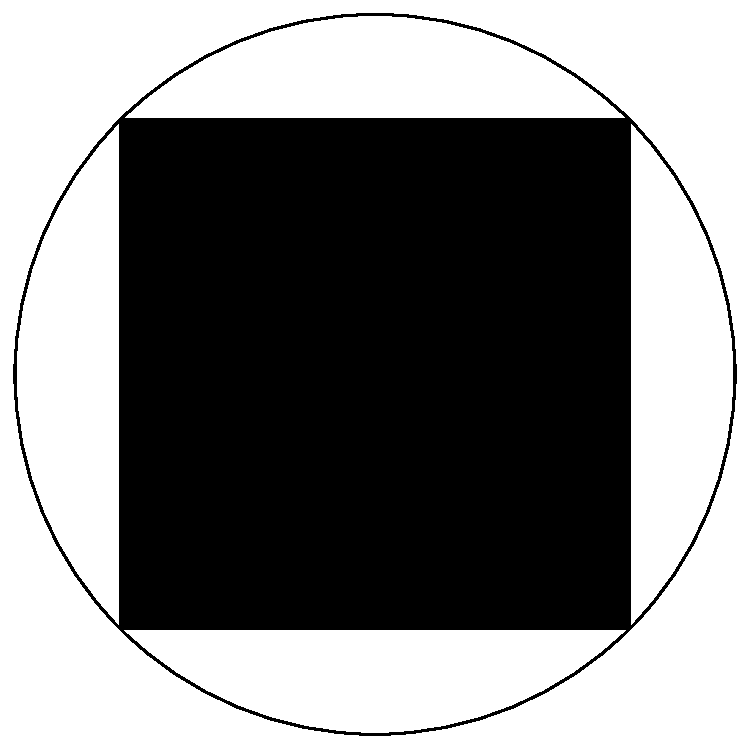
\includegraphics[scale=0.5]{Images/SquareP5.pdf}
				\caption{Cuadrado Inscrito en una Circunferecia, creado con \textit{Mathematica}.}
				\label{SP5}
			\end{figure}
			De modo que, el potencial debido a dichas cargas, en cualquier punto del espacio es:
			\begin{align*}
				\phi (x,y) &= \frac{1}{\sqrt{\left(x-\frac{a}{\sqrt{2}}\right)^2+\left(y+\frac{a}{\sqrt{2}}\right)^2}}+\frac{1}{\sqrt{\left(x+\frac{a}{\sqrt{2}}\right)^2+\left(y-\frac{a}{\sqrt{2}}\right)^2}} \\
				&+\frac{1}{\sqrt{\left(x-\frac{a}{\sqrt{2}}\right)^2+\left(y-\frac{a}{\sqrt{2}}\right)^2}}+\frac{1}{\sqrt{\left(x+\frac{a}{\sqrt{2}}\right)^2+\left(y+\frac{a}{\sqrt{2}}\right)^2}}
			\end{align*}
			Encontrando el campo eléctrico tomando el gradiente del potencial
			\begin{align*}
				\vec{E} &= \Bigg\{ \frac{x+\frac{a}{\sqrt{2}}}{\left(\left(x+\frac{a}{\sqrt{2}}\right)^2+\left(y+\frac{a}{\sqrt{2}}\right)^2\right)^{3/2}}+\frac{x+\frac{a}{\sqrt{2}}}{\left(\left(x+\frac{a}{\sqrt{2}}\right)^2+\left(y-\frac{a}{\sqrt{2}}\right)^2\right)^{3/2}} \\
				&+\frac{x-\frac{a}{\sqrt{2}}}{\left(\left(x-\frac{a}{\sqrt{2}}\right)^2+\left(y+\frac{a}{\sqrt{2}}\right)^2\right)^{3/2}}+\frac{x-\frac{a}{\sqrt{2}}}{\left(\left(x-\frac{a}{\sqrt{2}}\right)^2+\left(y-\frac{a}{\sqrt{2}}\right)^2\right)^{3/2}} \Bigg\} \vx \\
				&+\Bigg\{ \frac{y+\frac{a}{\sqrt{2}}}{\left(\left(x+\frac{a}{\sqrt{2}}\right)^2+\left(y+\frac{a}{\sqrt{2}}\right)^2\right)^{3/2}}+\frac{y+\frac{a}{\sqrt{2}}}{\left(\left(x-\frac{a}{\sqrt{2}}\right)^2+\left(y+\frac{a}{\sqrt{2}}\right)^2\right)^{3/2}} \\
				&+\frac{y-\frac{a}{\sqrt{2}}}{\left(\left(x+\frac{a}{\sqrt{2}}\right)^2+\left(y-\frac{a}{\sqrt{2}}\right)^2\right)^{3/2}}+\frac{y-\frac{a}{\sqrt{2}}}{\left(\left(x-\frac{a}{\sqrt{2}}\right)^2+\left(y-\frac{a}{\sqrt{2}}\right)^2\right)^{3/2}} \Bigg\} \vy
			\end{align*}
			Resolviendo por métodos numéricos se encontrarán $5$ soluciones, sin embargo este proceso ya es pesado y no se logró ejecutar completamente. Sin embargo, los puntos de campo cero convergen en la solución trivial $x,y= 0,0$.
			
			\item[Para $n = 5$: ] Se tiene que el potencial si se toma la figura como en la figura \ref{PP5}.
			\begin{figure}[H]
				\centering
				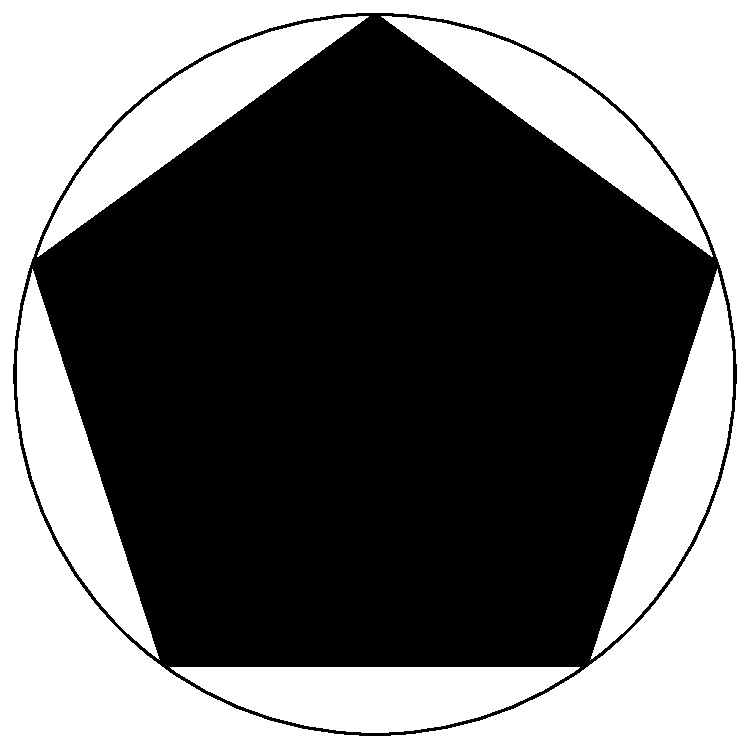
\includegraphics[scale=0.5]{Images/PentagonP5.pdf}
				\caption{Pentágono Inscrito en una Circunferecia, creado con \textit{Mathematica}.}
				\label{PP5}
			\end{figure}
			De modo que, el potencial debido a dichas cargas, en cualquier punto del espacio es:
				\begin{align*}
					\phi (x,y) &= \frac{q}{4\pi \varepsilon _o} \Bigg\{ \frac{1}{\sqrt{(y-a)^2+x^2}}+\frac{1}{\sqrt{(x-0.951 a)^2+(y-0.309 a)^2}} \\ 
					&+\frac{1}{\sqrt{(0.951 a+x)^2+(y-0.309 a)^2}}+\frac{1}{\sqrt{(x-0.588 a)^2+(0.809 a+y)^2}} \\ 
					&+\frac{1}{\sqrt{(0.588 a+x)^2+(0.809 a+y)^2}} \Bigg\}
				\end{align*}
			Con esto, se encuentra el campo:
				\begin{align*}
					\vec{E} &= \frac{q}{4\pi \varepsilon _o} \Bigg\{ \frac{x}{\left((y-a)^2+x^2\right)^{3/2}}+\frac{x-0.951 a}{\left((x-0.951 a)^2+(y-0.309 a)^2\right)^{3/2}} \\
					&+\frac{0.951 a+x}{\left((0.951 a+x)^2+(y-0.309 a)^2\right)^{3/2}}+\frac{x-0.588 a}{\left((x-0.588 a)^2+(0.809 a+y)^2\right)^{3/2}} \\ 
					&+\frac{0.588 a+x}{\left((0.588 a+x)^2+(0.809 a+y)^2\right)^{3/2}} \Bigg\} \vx \\
					& + \frac{q}{4\pi \varepsilon _o} \Bigg\{ \frac{y-a}{\left((y-a)^2+x^2\right)^{3/2}}+\frac{y-0.309 a}{\left((x-0.951 a)^2+(y-0.309 a)^2\right)^{3/2}} \\ 
					&+\frac{y-0.309 a}{\left((0.951 a+x)^2+(y-0.309 a)^2\right)^{3/2}}+\frac{0.809 a+y}{\left((x-0.588 a)^2+(0.809 a+y)^2\right)^{3/2}} \\ 
					&+\frac{0.809 a+y}{\left((0.588 a+x)^2+(0.809 a+y)^2\right)^{3/2}} \Bigg\} \vy
				\end{align*}
				
				Resolviendo por métodos numéricos: nos dará un conjunto de $6$ puntos, sin embargo, este es un proceso bastante pesado para las laptop, entonces ya no se logro ejecutar. Similar al poligono de cuatro vertices, los puntos convergen a $0,0$.
		\end{description}
		Para un $n\to \infty$ es claro que todos los puntos tienden a la solución trivial, el centro del círculo en el cual esta inscrito el poligono.
	\end{problem}
\end{mdframed}









% PROBLEMA 6
\begin{mdframed}[style = warning]
	\begin{problem}
		Incisos:
		\begin{enumerate}[a)]
			\item Encontrando la carga para cierto $r < R$, como se tiene simetría esférica y la carga no depende de los ángulos, entonces el diferencial de volumen se reduce a $\dd{V} = 4\pi r^2 \dd{r}$. Integrando:
				$$Q_{enc} = \int _0 ^r \frac{A}{r} (4\pi r^2) \dd{r} = 2\pi A r^2$$
			Aplicando la Ley de Gauss, la superficie gaussiana con el mismo radio $r$, se tiene:
				$$\boxed{\vec{E} = \frac{A}{2\varepsilon _o} \vr}$$
			Con esto, integrando se encuentra el potencial:
				$$\varphi (r) = -\int_{0} ^{r} \frac{1}{2} A \vr \cdot \vr \dd{r} = \boxed{-\frac{1}{2} Ar}$$
			Ahora, para $r\geq R$, se tiene que la carga encerrada es la carga total, con lo que, la integral se realiza desde $0$ hasta $R$:
				$$Q_{T} = 2\pi AR^2$$
			Con lo que el campo eléctrico es:
				$$\boxed{E(r\geq R) = \frac{AR^2}{2\varepsilon _o r^2} \vr}$$
			Para la región fuera de la carga, el punto de referencia del potencial esta en el infinito. Con lo que:
				$$\varphi (r \geq R) = -\int _\infty ^r \frac{AR^2}{2\varepsilon _o r^2} \dd{r} = \boxed{\frac{AR^2}{2\varepsilon _o r}}$$
			Con esta información, se puede encontrar el comportamiento del campo y potencial en ambas regiones, dados por las siguientes gráficas
				\begin{multicols}{2}
					\textbf{Campo Eléctrico:}
					\begin{figure}[H]
						\centering
						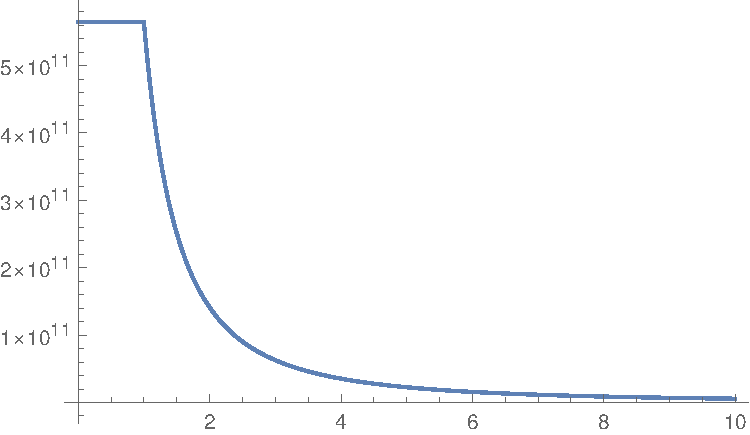
\includegraphics[scale=0.55]{Images/CampoP6a.pdf}
						\caption{Campo Eléctrico dentro y fuera de una esfera con densidad volumétrica de carga dada por $\flatfrac{A}{r}$.}
						\label{PP6a}
					\end{figure}
				\columnbreak
					\textbf{Potencial:}
					\begin{figure}[H]
						\centering
						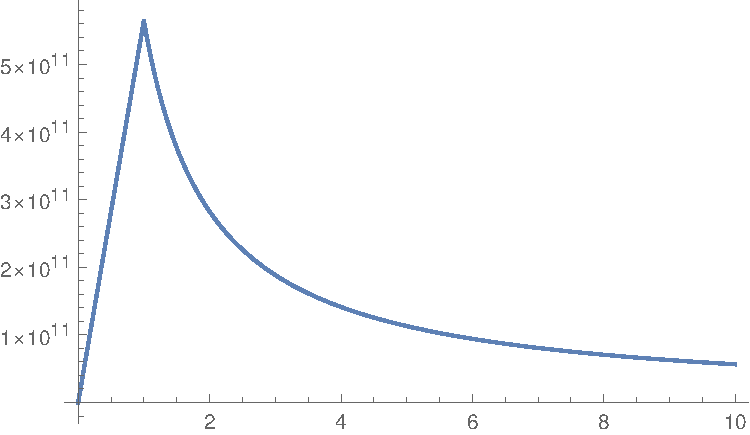
\includegraphics[scale=0.5]{Images/PotencialP6a.pdf}
						\caption{Potencial Eléctrico dentro y fuera de una esfera con densidad volumétrica de carga dada por $\flatfrac{A}{r}$.}
						\label{PP6a}
					\end{figure}
				\end{multicols}
			\item Para $\rho (r) = \rho _o$, se tiene que la carga encerrada en una superficie gaussiana de radio $r < R$ es:
				$$Q_{enc} = \frac{4}{3} \pi r^3 \rho _o$$
			Utilizando la ley de Gauss:
				$$\boxed{\vec{E} = \frac{\rho _o r}{3\varepsilon _o} \vr}$$
			Integrando, con el punto de referencia en cero, se encuentra el potencial:
				$$\boxed{\varphi (r < R) = -\frac{\rho _o r^2}{6\varepsilon _o}}$$
			Para $r \geq R$, la distribución se comporta como una carga puntual, por lo que el campo generado es:
				$$\boxed{\vec{E} = \frac{\rho _o R^3}{3 \varepsilon _o r^2} \vr}$$
			El potencial:
				$$\boxed{\varphi = \frac{\rho _o R^3}{3\varepsilon _o r}}$$
			Similarmente con el inciso anterior, se crean las gráficas para visualizar el comportamiento del campo y potencial entre regiones
				\begin{multicols}{2}
					\textbf{Campo Eléctrico:}
					\begin{figure}[H]
						\centering
						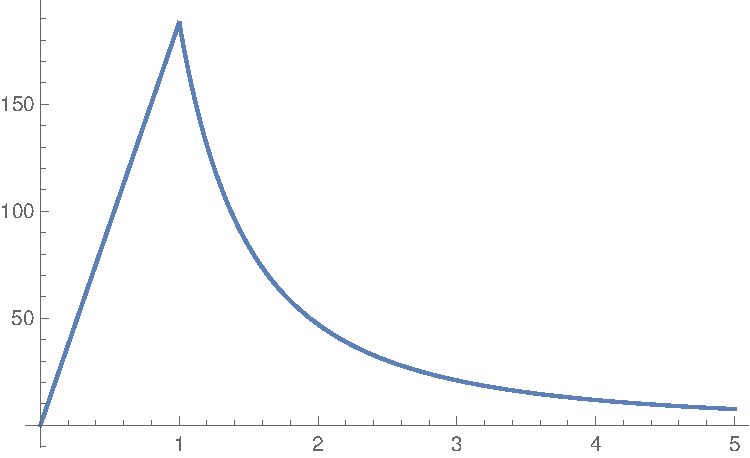
\includegraphics[scale=0.55]{Images/CampoP6b.pdf}
						\caption{Campo Eléctrico dentro y fuera de una esfera con densidad volumétrica de carga constante.}
						\label{PP6a}
					\end{figure}
				\columnbreak
					\textbf{Potencial:}
					\begin{figure}[H]
						\centering
						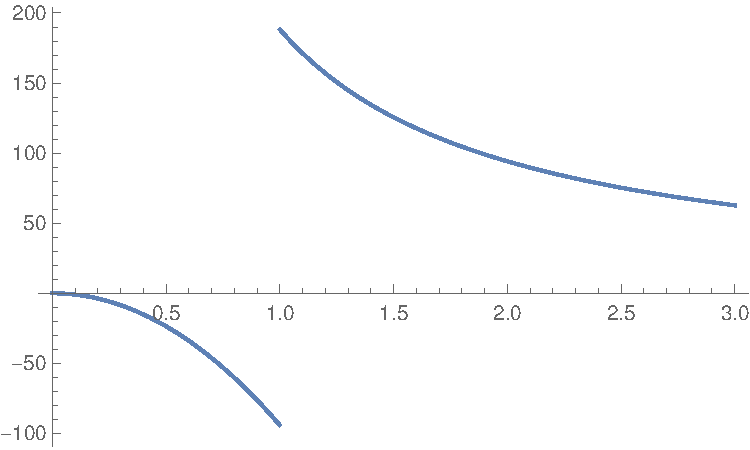
\includegraphics[scale=0.5]{Images/PotencialP6b.pdf}
						\caption{Potencial Eléctrico dentro y fuera de una esfera con densidad volumétrica de carga constante.}
						\label{PP6a}
					\end{figure}
				\end{multicols}
		\end{enumerate}
	\end{problem}
\end{mdframed}








% PROBLEMA 7
\begin{mdframed}[style = warning]
	\begin{problem}
		Utilizando la ley de Gauss (por siemtría en la distribución), se toma una superficie de un cilindro coaxial de radio $r < R$. Encontrando la carga encerrada por dicho cilindro es: ($\dd{V} = \pi r^2 \dd{z}$)
			$$Q_{enc} = \int _{\flatfrac{-l}{2}} ^{\flatfrac{l}{2}}\pi r^2 (\rho _o + \beta z) \dd{z}$$
		De modo que:
			$$Q_{enc} = \frac{\pi r^2 l}{\varepsilon _o} \rho _o$$
		El área de la superficie gaussiana es $A = 2\pi r l$
			$$\boxed{E(r<R) = \frac{\rho _o r}{2\varepsilon _o}}$$
	\end{problem}
\end{mdframed}








% PROBLEMA 8
\begin{mdframed}[style = warning]
	\begin{problem}
		Como es un cascarón esférico, el campo dentro, $r < R$, es cero. Por lo que, para un $z \geq R$ se tiene, utilizando la Ley de Gauss:
			$$Q_{enc} = \iint \sigma \dd{S} = \sigma (4\pi R^2) = q_T$$
		Por lo que, tomando una superficie gaussiana a una distancia $z$ del centro, se tiene:
			$$E(4\pi z^2) = \frac{q_T}{\varepsilon _o}$$
		De modo que:
			$$\boxed{\vec{E} = \frac{q_T}{4\pi \varepsilon _o} \frac{1}{z^2} \vz}$$
	\end{problem}
\end{mdframed}







% PROBLEMA 9
\begin{mdframed}[style = warning]
	\begin{problem}
		Para la configuración dada, se utiliza el método de las imagenes, de modo que:
		\begin{enumerate}[a)]
			\item La posición ideal del cilindro imagen es con un eje paralelo al cilindro original colocado en $-x_o$ y la carga de dicho cilindro igual a $-\lambda$.
			\item Realizando el procedimiento para dos cables paralelos ambos separados del centro del sistema de coordenadas una distancia $x_o$, con esto, se encuentra el campo eléctrico en cada punto, el cual se encontró en clase y se tiene:
				$$\vec{E} _\lambda = \frac{\lambda}{2\pi \varepsilon _o} \frac{\vec{r_1}}{r_1 ^2}$$
			De manera similar para la carga $-\lambda$ con $r_2$. De modo que, integrando se tiene que el potencial superpuesto es:
				$$\varphi _T = \frac{-\lambda}{2\pi \varepsilon _o} \ln{\frac{r_1}{r_2}}$$
			De modo que se toma a $M$ como:
				$$M = \frac{r_1}{r_2} = \frac{\sqrt{(x - x_o - a)^2 + y^2}}{\sqrt{(x + x_o + a)^2 + y^2}}$$
			Esto solo es válido para el lado de $+x_o$ y fuera del cilindro cargado. Con esto se tiene que, tomando a $M$ constante, se llega a la ecuación de un cilindro (cilindros equipotenciales), con esto y el desarrollo realizado en clase se tiene que el radio de dicho cilindro es:
				$$R_c = \frac{2Mx_o}{1 - M^2} = a$$
			Despejando	
				$$aM^2 + 2Mx_o - a = 0$$
			Resolviendo la ecuación cuadrática se tiene que $M$ tiene que valer:
				$$\boxed{M = \frac{-x_o \pm \sqrt{x_o ^2 - a^2}}{a}}$$
		\end{enumerate}
	\end{problem}
\end{mdframed}









% PROBLEMA 10
\begin{mdframed}[style = warning]
	\begin{problem}
		Incisos:
		\begin{enumerate}[a)]
			\item Para la región dentro del cilindro interior se tiene que el área de la superficie gaussiana es $2\pi r L$, el volumen $V = \pi r^2 L$, de modo que:
				$$\boxed{\vec{E} (r < a) = \frac{\rho r}{2\varepsilon _o} \vr}$$
			\item Para la región $a \leq r < b$, se utiliza la misma superficie gaussiana $E(2\pi r L)\varepsilon _o = \rho (\pi a^2 L)$, con lo que, el campo es:
				$$\boxed{\vec{E} (a \leq r < b) = \frac{\rho a^2}{2r\varepsilon _o} \vr}$$
			\item Como el cable en su totalidad es eléctricamente neutro, lo que implica que el campo eléctrico fuera del cable es cero:
				$$\boxed{\vec{E} (r \geq b) = 0}$$
		\end{enumerate}
		Con esta información, el campo eléctrico tiene un comportamiendo dado por la gráfica \ref{CP10}.
		\begin{figure}[H]
			\centering
			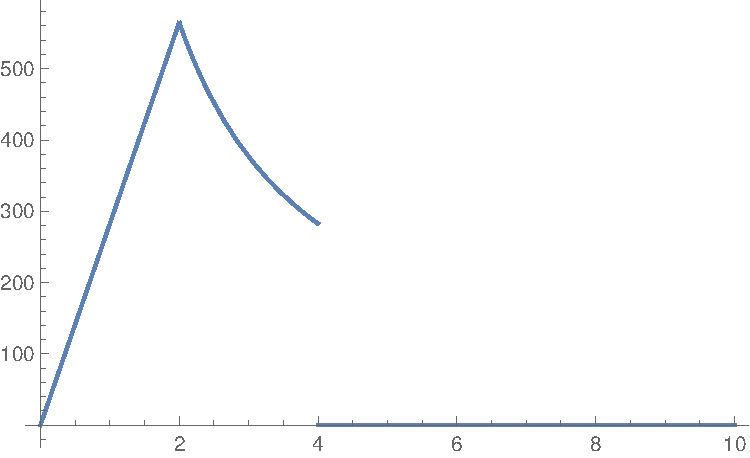
\includegraphics[scale=0.5]{Images/CampoP10.pdf}
			\caption{Campo Eléctrico definido por Regiones entre Cables Coaxiales}
			\label{CP10}
		\end{figure}
	\end{problem}
\end{mdframed}













